% Klassendeklaration
\documentclass[
		fontsize=12pt,		% Schriftgröße 12pt
		toc=listof,		% Schreibt Tabellen/Abbildungs-Verzeichnisse auch mit ins Inhaltsverzeichnis
		toc=bib,		% Literaturverzeichnis im Inhaltsverzeichnis aufführen
		%bibliography=openstyle	% Literaturverzeichnis etwas auflockern
		headsepline,		% Linie unter Kolumnentitel
		twoside=false,		% Layout für einseitigen Druck
		BCOR=12mm,		% Bindekorrektur: bei Buch normalerweise 12mm
		DIV=14,			% DIV-Wert fuer die Erstellung des Satzspiegels, siehe scrguide
		parskip=false,		% Absatzeinzug (Standard), half: kein Einzug, Halber Zeilenabstand, ...
		captions=tableheading,	% korrekte Abstände bei Tabellenüberschriften
		draft=false,		% true: Kennzeichnung von Absätzen, die manuell bearbeitet werden müssen, false: aus
		paper=A4,		% A4 Seite
		pagesize=automedia,	% Setzen der korrektern Papiergröße für Ausgabemedien
		numbers=noendperiod	% Auch wenn \appendix genutzt wird, keine Punkte hinter der Nummerierung (Regel im Duden sieht allerdings Punkt vor)
	]{scrbook}			% aus Komascript für Bücher
%%%%%%%%%%%%%%%%%%%%%%%%%%%%%%%%%%%%%%%%%%%%%%%%%%%%%%%%%%%%%%%%%%%%%%%%%%%%%%%%



% Pakete
\usepackage{cmap}		% to make the PDF files "searchable and copyable" in pdf viewer
\usepackage[english]{babel}	% deutschsprachig
\usepackage[utf8]{inputenc}	% utf8 encoding
\usepackage[T1]{fontenc}	% Schriftkodierung
\usepackage{lmodern}		% skalierbare Schriftfamilie "Latin Modern" (default: bitmapped "Computer Modern")
\usepackage{graphicx}		% Einbinden von Grafiken
\usepackage{booktabs}		% weitere Linien zur Strukturierung von Tabellen (\toprule, ...)
\usepackage{multirow}		% mehrere Zeilen in einer Tabelle zusammenfassen
\usepackage{ltxtable}		% longtable und tabularx vereint in einer Tabelle, lädt automatisch beide Pakete
\usepackage{rotating}		% Text drehen
\usepackage{amsmath}		% Matheumgebung
\usepackage{amssymb}		% Zusatzsymbole zB Square Vartriangle etc
\usepackage{moreverb}		% erweiterte verbatim Umgebung
\usepackage{listings}		% Listings -> Quellcodedarstellung für viele verschiedene Sprachen
\usepackage{subfigure}		% Unterbilder
\usepackage{xcolor}		% Farbdefinitionen möglich
\usepackage{pdfpages}		% Einbinden von PDF Seiten aus PDF Dokument
\usepackage{nicefrac}		% Darstellung eines Bruchs im Fließtext; Aussehen zB 1/4
\usepackage{acronym}		% Abkürzungsverzeichnis --> nur verwendete Abkürzungen listen [printonlyused]
\usepackage{bibgerm}		% deutsches Literaturverzeichnis
\usepackage{caption}		% viele caption Formatierungsmöglichkeiten
\usepackage{setspace}		% Zeilenabstand festlegen
\usepackage{microtype}		% Verbessert Textsatz
\usepackage{fixltx2e}		% Verbessert einige Kernkompetenzen von LaTeX2e
\usepackage{ellipsis}		% Korrigiert den Weißraum um Auslassungspunkte
\usepackage{units}		% Einheiten komfortabel darstellen \unit[Zahlenwert]{Einheit}
\usepackage{textcomp}		% einige Text-Mode Mathe Symbole, wie zB Mal-Zeichen x (siehe The Comprehensive LaTeX Symbol List)
\usepackage{gensymb}		% celsius, micro, ohm, perthousand, degree in Mathe und Textmodus
%%%%%%%%%%%%%%%%%%%%%%%%%%%%%%%%%%%%%%%%%%%%%%%%%%%%%%%%%%%%%%%%%%%%%%%%%%%%%%%%

% Einbindung von allen Grafikformaten möglich
\usepackage{pst-pdf} % pstricks und ps grafiken in pdflatex
\usepackage{pst-all}
\usepackage{pstricks-add}
%%%%%%%%%%%%%%%%%%%%%%%%%%%%%%%%%%%%%%%%%%%%%%%%%%%%%%%%%%%%%%%%%%%%%%%%%%%%%%%%


% für Fließumgebungen
% Platzierung H zwingt LaTeX Fließumgebungen genau an diese Stelle zu setzen
\usepackage{float}
\usepackage{wrapfig}
%%%%%%%%%%%%%%%%%%%%%%%%%%%%%%%%%%%%%%%%%%%%%%%%%%%%%%%%%%%%%%%%%%%%%%%%%%%%%%%%


% Kopf- und Fußzeilen
\usepackage[headsepline]{scrpage2}	% Paket, Linie unter Kopfangabe
\clearscrheadfoot			% löscht alle bisherigen Kopf- und Fußzeilen
\pagestyle{scrheadings}			% selbstgebastelte Kopf-/Fußzeilen
\automark{chapter}			% \automark[<rechte seite>]{<linke seite>}
\ihead{\leftmark}			% setzt Kopfzeile (chapterangabe)
\cfoot[-\,\pagemark\,-]{-\,\pagemark\,-}% setzt Fußzeile [] -> chapterseiten; {} -> alle anderen Seiten
%%%%%%%%%%%%%%%%%%%%%%%%%%%%%%%%%%%%%%%%%%%%%%%%%%%%%%%%%%%%%%%%%%%%%%%%%%%%%%%%



% Schusterjungen und Hurenkinder vermeiden
\clubpenalty = 10000
\widowpenalty = 10000
\displaywidowpenalty = 10000
%%%%%%%%%%%%%%%%%%%%%%%%%%%%%%%%%%%%%%%%%%%%%%%%%%%%%%%%%%%%%%%%%%%%%%%%%%%%%%%%



% Farbdefinitionen
\definecolor{fill}{rgb}{1,1,0.73}
%%%%%%%%%%%%%%%%%%%%%%%%%%%%%%%%%%%%%%%%%%%%%%%%%%%%%%%%%%%%%%%%%%%%%%%%%%%%%%%%




% Workaround eines Bugs des wrapfig Paketes
% Entfernen wenn neue Version den Pakets verfügbar ist
% wenn ein umflossenes Bild nicht vollständig umflossen wird
% muss der Absatz geschlossen werden: dazu dann den Befehl
% \wrapfill hinter dem Absatz notieren
\usepackage{blindtext,wrapfig}
\makeatletter
\newcommand\wrapfill{\par
    \ifx\parshape\WF@fudgeparshape
    \nobreak
    \vskip-\baselineskip
    \vskip\c@WF@wrappedlines\baselineskip
    \allowbreak
    \WFclear
    \fi
}
\makeatother
%%%%%%%%%%%%%%%%%%%%%%%%%%%%%%%%%%%%%%%%%%%%%%%



% interne und externe Links werden als Hyperlinks übersetzt
% viele andere Optionen für pdf viewer möglich
% pdf metadaten
\usepackage{hyperref}
\hypersetup{pdftitle={Master thesis - Modelling and simulation of electricity generation from run-of-the-river hydroelectric power plants based on open access geodatabases},
	pdfauthor={Chloe Lucas},
	pdfsubject={Modelling and simulation of electricity generation from run-of-the-river hydroelectric power plants based on open access geodatabases},
	pdfcreator={LaTeX (TexLive 2008)},
	pdfproducer={LaTeX (TexLive 2008)},
	pdfkeywords={key, word},
	colorlinks=true,
	urlcolor=black,
	linkcolor=black,
	citecolor=black,
	unicode=true
}
%%%%%%%%%%%%%%%%%%%%%%%%%%%%%%%%%%%%%%%%%%%%%%%%%%%%%%%%%%%%%%%%%%%%%%%%%%%%%%%%


% caption setup
% hang: bereich unter dem bezeichner bleibt frei;
% figurename: Bezeichner umdefinieren;
% margin: Einzug links und rechts
\captionsetup{format=hang,margin=30pt}
\captionsetup[lstlisting]{skip=13pt}
%%%%%%%%%%%%%%%%%%%%%%%%%%%%%%%%%%%%%%%%%%%%%%%%%%%%%%%%%%%%%%%%%%%%%%%%%%%%%%%%



%% Listings-Formatierung
\lstset{%
	language=vbscript, %
	basicstyle=\tiny,%\scriptsize,
	frame=trbl,%
	numbers=left,%
	breaklines=true,
	prebreak=\mbox{$\hookleftarrow$},
	postbreak=\mbox{$\longrightarrow$},
	breakatwhitespace=true,
	captionpos=t,%
	showstringspaces=false,
	numberstyle=\tiny,%
	commentstyle=\color{red},%
	keywordstyle=\bfseries\color{blue},%
	backgroundcolor=\color{fill},%
	rulecolor=\color{gray}%
}
%%%%%%%%%%%%%%%%%%%%%%%%%%%%%%%%%%%%%%%%%%%%%%%%%%%%%%%%%%%%%%%%%%%%%%%%%%%%%%%%



% Tabellen
% neuer Spaltentyp C --> zentrierte X Spalten
\newcolumntype{C}{>{\centering\arraybackslash}X}
% Größere Höhe von Tabellenzellen
\renewcommand{\arraystretch}{1.3}
%%%%%%%%%%%%%%%%%%%%%%%%%%%%%%%%%%%%%%%%%%%%%%%%%%%%%%%%%%%%%%%%%%%%%%%%%%%%%%%%



% chapterüberschriften ohne Abstand zum Kopf festlegen
% \renewcommand*{\chapterheadstartvskip}{\vspace*{-\topskip}}
%%%%%%%%%%%%%%%%%%%%%%%%%%%%%%%%%%%%%%%%%%%%%%%%%%%%%%%%%%%%%%%%%%%%%%%%%%%%%%%%



% 1,5-Zeilenabstand (Paket setspace erforderlich)
\onehalfspacing
% Neuberechnung des Satzspiegels für neuen Zeilenabstand (DIV Angabe aus der
% Klassendeklartion übernommen)
\KOMAoptions{DIV=last}
%%%%%%%%%%%%%%%%%%%%%%%%%%%%%%%%%%%%%%%%%%%%%%%%%%%%%%%%%%%%%%%%%%%%%%%%%%%%%%%%



% Befehle für Hoch und Tiefstellen innerhalb eines Textes
\newcommand{\up}[2]{#1\textsuperscript{#2}}
\newcommand{\down}[2]{#1\textsubscript{#2}}
%%%%%%%%%%%%%%%%%%%%%%%%%%%%%%%%%%%%%%%%%%%%%%%%%%%%%%%%%%%%%%%%%%%%%%%%%%%%%%%%



% Beginn des Dokuments
\begin{document}

	%Vorspann
	\frontmatter

	% große römische Ziffern für die Seitennummern im Vorspann (Standard sind kleine römische Ziffern)
	\pagenumbering{Roman}

	% Includes Vorspann
	% Titelseite
	%%%%%%%%%%%%%%%%%%%%%%%%%%%%%%%%%%%%%%%%%%%%%%%%%%%%%%%%%%%%%%
% \titlehead	Kopfzeile der Titelseite
% \subject	Thema des Dokumentes
% \title	Titel des Dokumentes
% \subtitle	Untertitel
% \author	Autor des Dokumentes
% \date	Datum der Veröffentlichung
% \dedication	Widmung ;-)
% \publishers	Herausgeber
% \thanks	Fußnote
% \begin{abstract}
%   ...
% \end{abstract}

\newcommand{\mytitle}{}
\newcommand{\setmytitle}[1]{\renewcommand{\mytitle}{#1}}

\newcommand{\myauthor}{}
\newcommand{\setmyauthor}[1]{\renewcommand{\myauthor}{#1}}

\newcommand{\mysubject}{}
\newcommand{\setmysubject}[1]{\renewcommand{\mysubject}{#1}}


\setmytitle{Modelling and simulation of electricity generation from run-of-the-river hydroelectric power plants based on open access geodatabases}
\setmyauthor{Chloë Lucas}
\setmysubject{Master Thesis}

\titlehead{%
	\fontsize{14pt}{12} \selectfont%
	\textbf{Technische Universität Berlin} \\%
	\vspace{0.5cm}%
	Institute for Energy Engineering
}

\title{}
\subject{\hrulefill \\
	\vspace{0.1cm}%
	\mysubject \\
	\vspace{0.5cm}%
	\mytitle \\% 
	\hrulefill
	\vspace{-1cm}%
}
\author{%
	{
	\renewcommand{\arraystretch}{1}
	\fontsize{12pt}{12} \selectfont%
	\begin{tabular}{lcl}%
		Submitted by & : & \myauthor \\%		
		Student ID & : & 376567 \\%
	\end{tabular}
	}\\[2cm]%
	{
	\renewcommand{\arraystretch}{1}
	\fontsize{12pt}{12} \selectfont%
 	\begin{tabular}{lcl}
		External supervisor & : & Msc. Birgit Schachler \\%
		& &Reiner Lemoine Institute \\%
		\\
		Reviewers& :& Dipl.-Ing. Mathias Hofmann \\%
		& &Technische Universität Berlin\\%
		\\
 		& & Prof. Dr.-Ing. George Tsatsaronis\\%
		& &Technische Universität Berlin\\%
		\\%
	\end{tabular}%	
	}\\[3cm]
	{
	\fontsize{12pt}{12} \selectfont%
	\textbf{\today, Berlin}
	}
}
\date{}

%%%%%%%%%%%%%%%%%%%%%%%%%%%%%%%%%%%%%%%%%%%%%%%%%%%%%%%%%%%%%%%%
\maketitle
	%%%%%%%%%%%%%%%%%%%%%%%%%%%%%%%%%%%%%%%%%%%%%%%%%%%%%%%%%%%%%%%%%%%%%%%%%%%%%%%%
	% offizielle Aufgabenstellung
%	\include{./chapter/aufgabenstellung}
	%%%%%%%%%%%%%%%%%%%%%%%%%%%%%%%%%%%%%%%%%%%%%%%%%%%%%%%%%%%%%%%%%%%%%%%%%%%%%%%%
	% Selbstständigkeitserklärung
	\chapter*{Declaration of authorship}

I, \myauthor, hereby declare that this \mysubject\ submitted at the faculty III on the topic of
\vspace{0.5cm}
\begin{center}
	\textbf{\mytitle}
\end{center}
\vspace{0.5cm}
and the work presented in it are my own and has been generated by me as the result of my own original research, unless stated otherwise. No other person’s work has been used without due acknowledgement and all references have been quoted.
\\[4ex]
Berlin, \today \\
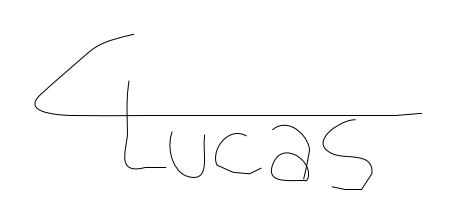
\includegraphics[width=3cm]{signature.png}
\\[-4ex] \newline
\myauthor

	%%%%%%%%%%%%%%%%%%%%%%%%%%%%%%%%%%%%%%%%%%%%%%%%%%%%%%%%%%%%%%%%%%%%%%%%%%%%%%%%
	% Inhaltsverzeichnis
	\tableofcontents
	%%%%%%%%%%%%%%%%%%%%%%%%%%%%%%%%%%%%%%%%%%%%%%%%%%%%%%%%%%%%%%%%%%%%%%%%%%%%%%%%
	% Abbildungsverzeichnis
	\listoffigures
	%%%%%%%%%%%%%%%%%%%%%%%%%%%%%%%%%%%%%%%%%%%%%%%%%%%%%%%%%%%%%%%%%%%%%%%%%%%%%%%%
	% Tabellenverzeichnis
	\listoftables
	%%%%%%%%%%%%%%%%%%%%%%%%%%%%%%%%%%%%%%%%%%%%%%%%%%%%%%%%%%%%%%%%%%%%%%%%%%%%%%%%
	% Listings-Verzeichnis
%	\renewcommand{\lstlistlistingname}{Quelltexte}
%	\lstlistoflistings
	%%%%%%%%%%%%%%%%%%%%%%%%%%%%%%%%%%%%%%%%%%%%%%%%%%%%%%%%%%%%%%%%%%%%%%%%%%%%%%%%
	% Abkürzungsverzeichnis/Formelzeichen
	\chapter*{List of Abbreviations}

\begin{acronym}
\small
\itemsep0em
\acro{AEE}{Agentur für Erneuerbare Energien}
\acro{BfG}{German Federal Institute of Hydrology - Bundesanstalt für Gewässerkunde}
\acro{BNetzA}{Federal Network Agency - Bundesnetzagentur}
\acro{CETMEF}{Center for Maritime and Fluvial Studies - Centre d'Études Techniques Maritimes et Fluviales}
\acro{DGJ}{Deutsches Gewässerkundliches Jahrbuch}
\acro{DLM250}{Digital Landscape Model 1:250000}
\acro{EEG}{German Renewable Energy Sources Act - Erneuerbare-Energien-Gesetz}
\acro{GHG}{Greenhouse Gas}
\acro{GIS}{Geographic Information System}
\acro{GRDC}{Global Runoff Data Center}
\acro{GWK}{River identification number - Gewässerkennzahl}
\acro{MaStR}{Marktstammdatenregister}
\acro{OECD}{Organisation for Economic Co-operation and Development}
\acro{OEDB}{OpenEnergy DataBase}
\acro{openFRED}{open Feed-in time series based on a Renewable Energy Database}
\acro{OPDS}{Open Power Data Set}
\acro{ROR}{Run-Of-the-River}
\acro{WSV}{Federal Waterways and Shipping Administration - Wasserstraßen- und Schifffahrtsverwaltung des Bundes}
\acro{German federal states :}{}
\acro{B}{Berlin}
\acro{BB}{Brandenburg}
\acro{BW}{Baden-Württemberg}
\acro{BY}{Bavaria}
\acro{HB}{Bremen}
\acro{HE}{Hesse}
\acro{HH}{Hamburg}
\acro{MV}{Mecklenburg-Vorpommern}
\acro{NI}{Lower Saxony}
\acro{NW}{North Rhine-Westphalia}
\acro{RLP}{Rhineland-Palatinate}
\acro{SH}{Schleswig-Holstein}
\acro{SL}{Saarland}
\acro{SN}{Saxony}
\acro{ST}{Saxony-Anhalt}
\acro{TH}{Thuringia}
\end{acronym}
	%%%%%%%%%%%%%%%%%%%%%%%%%%%%%%%%%%%%%%%%%%%%%%%%%%%%%%%%%%%%%%%%%%%%%%%%%%%%%%%%
	%%%%%%%%%%%%%%%%%%%%%%%%%%%%%%%%%%%%%%%%%%%%%%%%%%%%%%%%%%%%%%%%%%%%%%%%%%%%%%%%

	% Hauptteil
	\mainmatter

	\chapter{Introduction}
\label{chap:introduction}

\section{Energy systems modelling}

In the past decades, the need for an energy transition has emerged in many countries. This need has been acknowledge in the sustainable development goals \cite{un_sdgs} set by the United Nations, in particular the goals 7 \cite{un_sdg7} and 11 \cite{un_sdg11} : ``affordable and clean energy'' and ``sustainable cities and communities''. However, a successful energy transition will have a positive impact on other development goals as well, through a reduction of pollution, global warming, and conflicts about the access to fosil fuels. \newline
The transition in the production of energy is made possible by replacing conventional fuels such as coal, gas or uranium by renewable energy sources, such as wind, sunlight, kinetic and potential energy of water, geothermal energy or biomass. These energy sources are harnessed on site, and the potential of a site is highly dependant on the weather, the relief, as well as the time of the year or of the day. This leads to a more decentralized and intemittent production compared to conventional power plants, which complexifies the energy system. \newline
Because of the intermittency of the production and the strong dependance on weather, the energy supply is not controllable, and cannot always follow the demand. Furthermore, the variablility in the potential of each type of renewable energy depending on the site make it impossible to have a general solution applicable everywhere. This prompts the need for reliable energy systems modelling to simulate and optimize the energy mix, distribution schema and energy management of a given region. The simulation of energy systems requires good quality energy conversion and distribution models, consistent data about the weather, the existing plants in the region, and the energy demand, and robust optimisation tools.


\section{Open source}

The volume of research about renewable energy has grown over the last decades (more than 180 university and 120 non-university research institutes are conducting research about energy transition in Germany alone \cite{bmbf_energiewende}), and various actors of the energy sector are developping models for energy systems and gathering input data for these models. The complexity of the models has also increased, requiring specialists of differents fields to work together (geographers, meteorologists, energy specialists, economists, sociologists,etc). A wide range of case studies can be found in research articles, exposing the methods used and the results of these models for specific regions. However the tools themselves are rarely made public, which forces different actors to inject time, money and energy into developping the same models and gathering the same data. \newline
The Open Energy Modelling initiative (Openmod) was launched in september 2014 by several researchers in Germany and abroad \cite{openmod_workshop} and aims at promoting open energy modelling in Europe. They define “Open” as model source code that can be studied, changed and improved as well as freely available energy system data and state that more openness in energy modelling will increase transparency and credibility, reduce wasteful double-work and improve overall quality \cite{openmod_manifesto}. \newline
The Reiner Lemoine institute has been part of this initiative since the beginning and  carries out several projects of open energy modelling, such as oemof (open energy system modelling framework \cite{rli_oemof}), open\_eGo (open electricity grid optimisation \cite{rli_openego}) or open\_FRED (open feed-in time series based on a renewable energy database \cite{rli_openfred}). This thesis is part of the open\_FRED project, which aims at creating and making available in an open data base consistent standard data of all relevant data sets (power plant, climate, and basic data), and at developping compatible open source simulations models, which will produce feed-in time series of fluctuating renewable energies. \newline
The topic of this thesis is the modelling and simulation of electricity generation from run-of-the-river hydroelectric power plants based on open access geodatabases. It aims at developping an open-source Python model able to simulate time series of the electrical output of one or several run-of-the-river power plants based on open source datasets of power plants, weather, and river discharge.


\section{Hydropower}
Hydropower in the world \newline
Hydropower in Europe (example Norway?) \newline
Hydropower in Germany (places, part of the mix, installed capacity, potential) \newline
Pros and cons and ror vs not ror \newline





	%% hier eigentliche Kapitel einfügen

	\chapter*{Abstract}
\label{chap:abstract}

	%%%%%%%%%%%%%%%%%%%%%%%%%%%%%%%%%%%%%%%%%%%%%%%%%%%%%%%%%%%%%%%%%%%%%%%%%%%%%%%%

	% Anhang
	\appendix
\chapter{Source code}
\label{app:source_code}

\lstinputlisting[caption={Source code}, label=lst:source_code]
	{./data/test.txt}
	%%%%%%%%%%%%%%%%%%%%%%%%%%%%%%%%%%%%%%%%%%%%%%%%%%%%%%%%%%%%%%%%%%%%%%%%%%%%%%%%


	% Literaturverzeichnis
	% Preambel für das Literaturverzeichnis
	\setbibpreamble{The bibliography is sorted alphabetically based on the authors names. In the case of several authors, the work is sorted based on the first author.  \par\bigskip}
	\bibliography{./bibliography/verzeichnis.bib}{} % Datei
	% Layout
	\bibliographystyle{plain}
	% alle Literaturangaben (auch unzitierte)
	\nocite{*}
	% Info: Autoren mit AND trennen, wenn genaue Formatierung ohne Umsortierung gewünscht dann ...= "{...}"
	%%%%%%%%%%%%%%%%%%%%%%%%%%%%%%%%%%%%%%%%%%%%%%%%%%%%%%%%%%%%%%%%%%%%%%%%%%%%%%%%

% Dokumentende
\end{document}
